\subsubsection{Melt migration in a 2D mid-ocean ridge model}
\label{sec:cookbooks-mid-ocean-ridge}

\textit{This section was contributed by Juliane Dannberg.}

The following cookbook will explain how to set up a model of a mid-ocean ridge that uses \aspect{}'s
implementation of coupled magma/mantle dynamics (see Section~\ref{sec:melt_transport}) and melting
and freezing of mantle rock.
In particular, it will outline
\begin{enumerate}
  \item how to use operator splitting to accurately compute melting and freezing of melt,
  \item how to use traction boundary conditions to set up the flow field of a mid-ocean ridge,
  \item useful strategies for how to refine the mesh in models with melt migration.
\end{enumerate}
How to set up a model with melt migration in general is explained in the previous cookbook \ref{sec:cookbooks-melt-global}.

As the flow at mid-ocean ridges can be assumed to be roughly symmetric with respect to the ridge axis
in the center, we only model one half of the ridge in a 2d Cartesian box with dimensions of $105 \times 70$\,km. Solid material is flowing in from the bottom with a prescribed temperature and melting due to decompression as is rises. The model is cooled from the top so that melt freezes again as it approaches this boundary. In addition, a fixed plate velocity away from the ridge axis is prescribed at the top boundary, inducing corner flow. Material can flow out freely at the right model boundary. The model shows both how melt is focused towards the ridge axis, and how melting and freezing induces chemical heterogeneity in the mantle, generating the crust and lithosphere.
A movie of the full model evolution can be found \href{https://www.youtube.com/watch?v=f4Bc4lzdNP0}{online}.

\paragraph{The input file.}
One important problem in models with melting and freezing (and other reactions) is that these reactions
can be much faster than the time step of the model. For mid-ocean ridges, melt is generally assumed to
be in equilibrium with the solid, which means that the reaction is basically instantaneous.
To model these type of processes, \aspect{} uses operator splitting (see also Section \ref{sec:benchmark-operator_splitting}): Reactions are solved on a different time scale than advection.
For this model, this means that at the beginning of each time step, all melting reactions,
including their latent heat effects, are solved using several shorter sub-time steps. In the input file,
we have to choose both the size of these sub-time steps and the rate (or characteristic time scale) of melting,
and they have to be consistent in the sense that the operator splitting time step can not be larger than
the reaction time scale.
The melting model we use here is the anhydrous mantle melting model of \cite{KSL2003} for a peridotitic
rock composition, as implemented in the ``melt simple'' material model.

\lstinputlisting[language=prmfile]{cookbooks/mid_ocean_ridge/doc/melting_and_freezing.part.prm.out}

To make sure we reproduce the characteristic triangular melting region of a mid-ocean ridge, we have to
set up the boundary conditions in a way so that they will lead to corner flow. At the top boundary, we can
simply prescribe the half-spreading rate, and at the left boundary we can use a free-slip boundary, as
material should not cross this centerline. However, we do not know the inflow and outflow velocities at
the bottom and right side of the model. Instead, what we can do here is prescribing the lithostatic
pressure as a boundary condition for the stress. We accomplish this by using the
``initial lithostatic pressure'' model. This plugin will automatically compute a 1d lithostatic pressure
profile at a given point at the time of the model start and apply it as a boundary traction.

\lstinputlisting[language=prmfile]{cookbooks/mid_ocean_ridge/doc/boundary_conditions.part.prm.out}

Finally, we have to make sure that the resolution is high enough to model melt migration.
This is particularly important in regions where the porosity is low, but still high enough that
the two-phase flow equations are solved (instead of the Stokes system, which is solved if there is
no melt present in a cell). At the boundary between these regions, material properties like the
compaction viscosity may jump, and there may be strong gradients or jumps in some solution variables such
as the melt velocity and the compaction pressure. In addition, the characteristic length scale for melt transport,
the compaction length $\delta$, depends on the porosity:
\begin{equation}
\delta = \sqrt{\frac{(\xi+4\eta/3)k}{\eta_f}}.
\end{equation}
While the melt viscosity $\eta_f$ is usually assumed to be constant, and the shear and compaction
viscosities $\eta$ and  $\xi$ increase with decreasing porosity $\phi$, the permeability
$k \propto \phi^2$ or $k \propto \phi^3$ dominates this relation, so that the compaction length becomes
smaller for lower porosities.
As the length scale of melt migration is usually smaller than for mantle convection, we want to make
sure that regions where melt is present have a high resolution, and that this high resolution extends
to all cells where the two-phase flow equations are solved.

\lstinputlisting[language=prmfile]{cookbooks/mid_ocean_ridge/doc/mesh_refinement.part.prm.out}

\aspect{} also supports an alternative method to make sure that regions with melt are sufficiently
well resolved, relying directly on the compaction length, and we will discuss this method as a possible
modification to this cookbook at the end of this section.

The complete input file is located at \url{cookbooks/mid_ocean_ridge/mid_ocean_ridge.prm}.

\paragraph{Model evolution.}

\begin{figure}
    \centering
    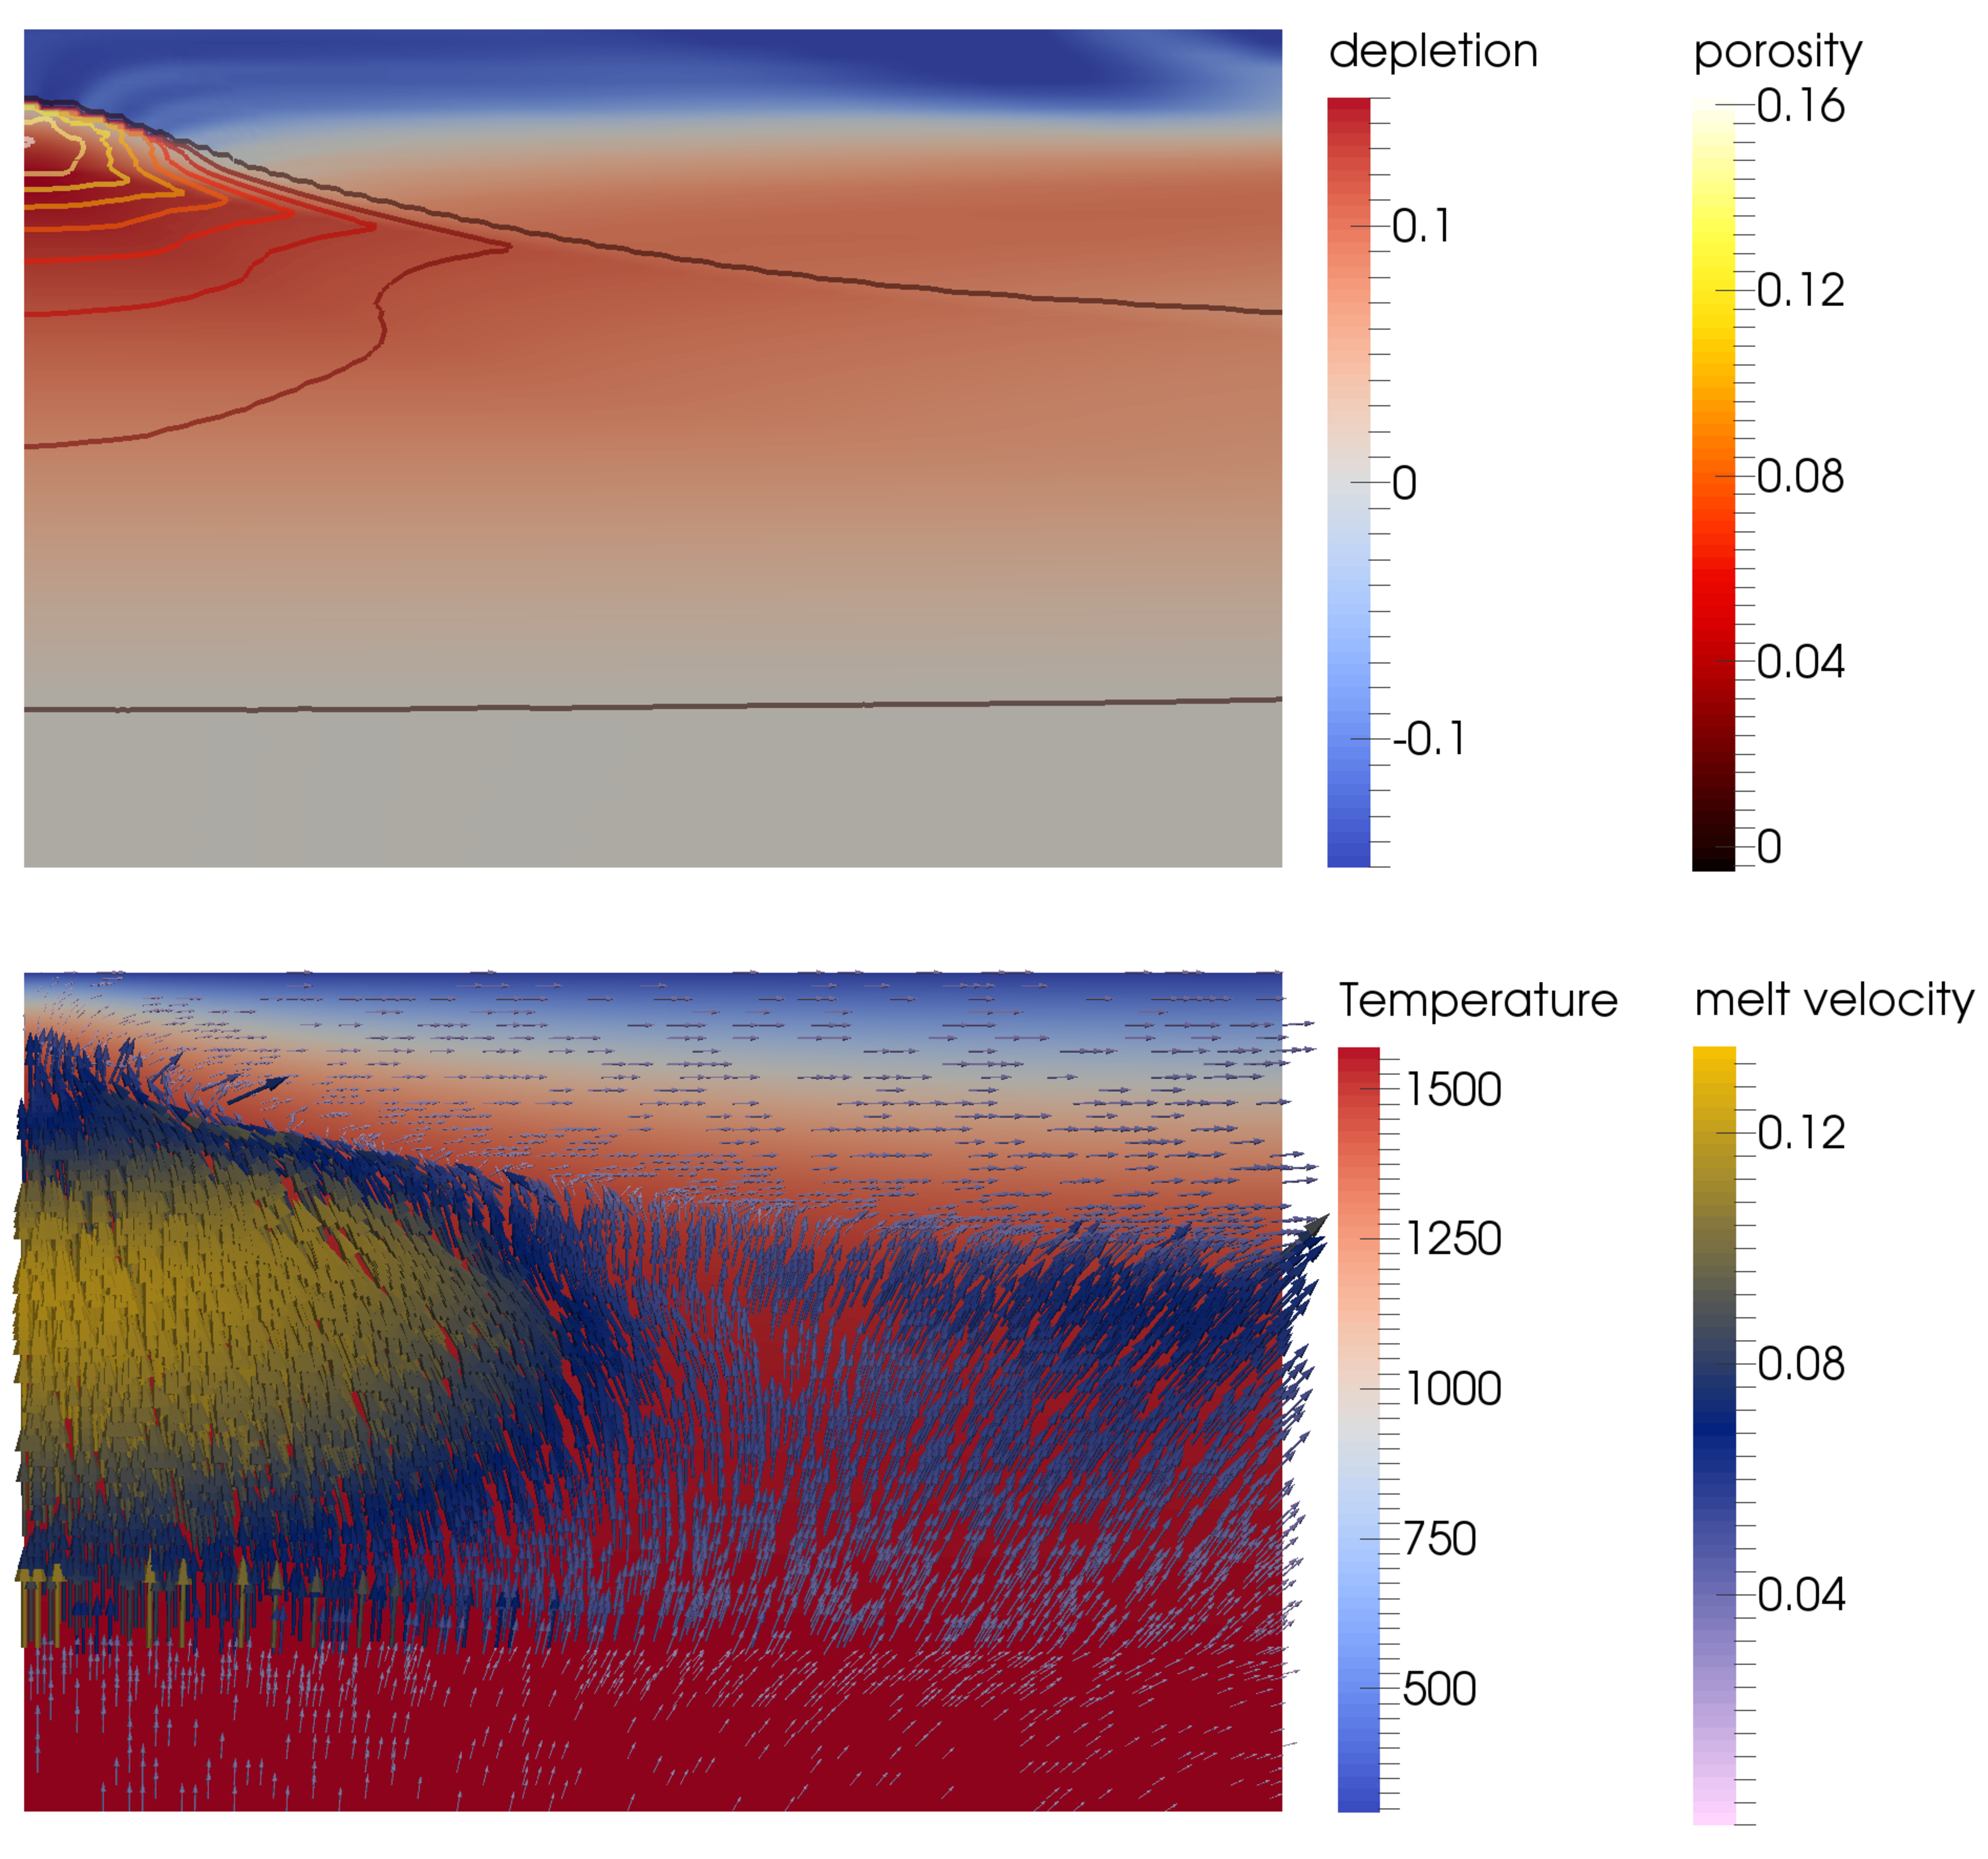
\includegraphics[width=0.5\textwidth]{cookbooks/mid_ocean_ridge/doc/mid_ocean_ridge.pdf}
    \caption{\it Mid-ocean ridge model after 8 million years. The top panel shows the depletion
             and porosity fields (with the characteristic triangular melting region),
             the bottom panel shows the temperature distribution and the melt velocity, indicated
             by the arrows.}
    \label{fig:mid-ocean-ridge}
\end{figure}

When we look at the visualization output of this model (see also Figure~\ref{fig:mid-ocean-ridge}),
we can see how the hot material flowing in
from the bottom starts to melt as it reaches lower and lower pressures and crosses the solidus.  Simultaneously, melting makes the residual solid rock more depleted (as indicated by the positive
values of the compositional field called `peridotite'). Once material approaches the surface,
it is cooled from the cold boundary layer above, and melt starts to crystallize again, generating
`enriched' basaltic crust where is freezes (as indicated by the negative values of the compositional
field called `peridotite'). As the temperature gradients are much sharper close to the surface, this
transition from melt to solid rock is much sharper than in the melting region. Once material
crystallizes, it is transported away from the ridge axis due to the flow field induced by the prescribed
plate velocity at the top boundary. This way, over time, the classical triangular melting region develops
at the ridge axis, and the material transported away from the ridge shows two distinct layers:
The top $\approx 7$ km are enriched material, and form the basaltic crust (negative peridotite field),
and the $\approx 50$ km below are depleted material, and form the lithosphere (positive peridotite field).
A vertical profile at a distance of 80 km from the ridge axis showing this composition can be found in Figure~\ref{fig:mid-ocean-ridge-profile}.

\begin{figure}
    \centering
    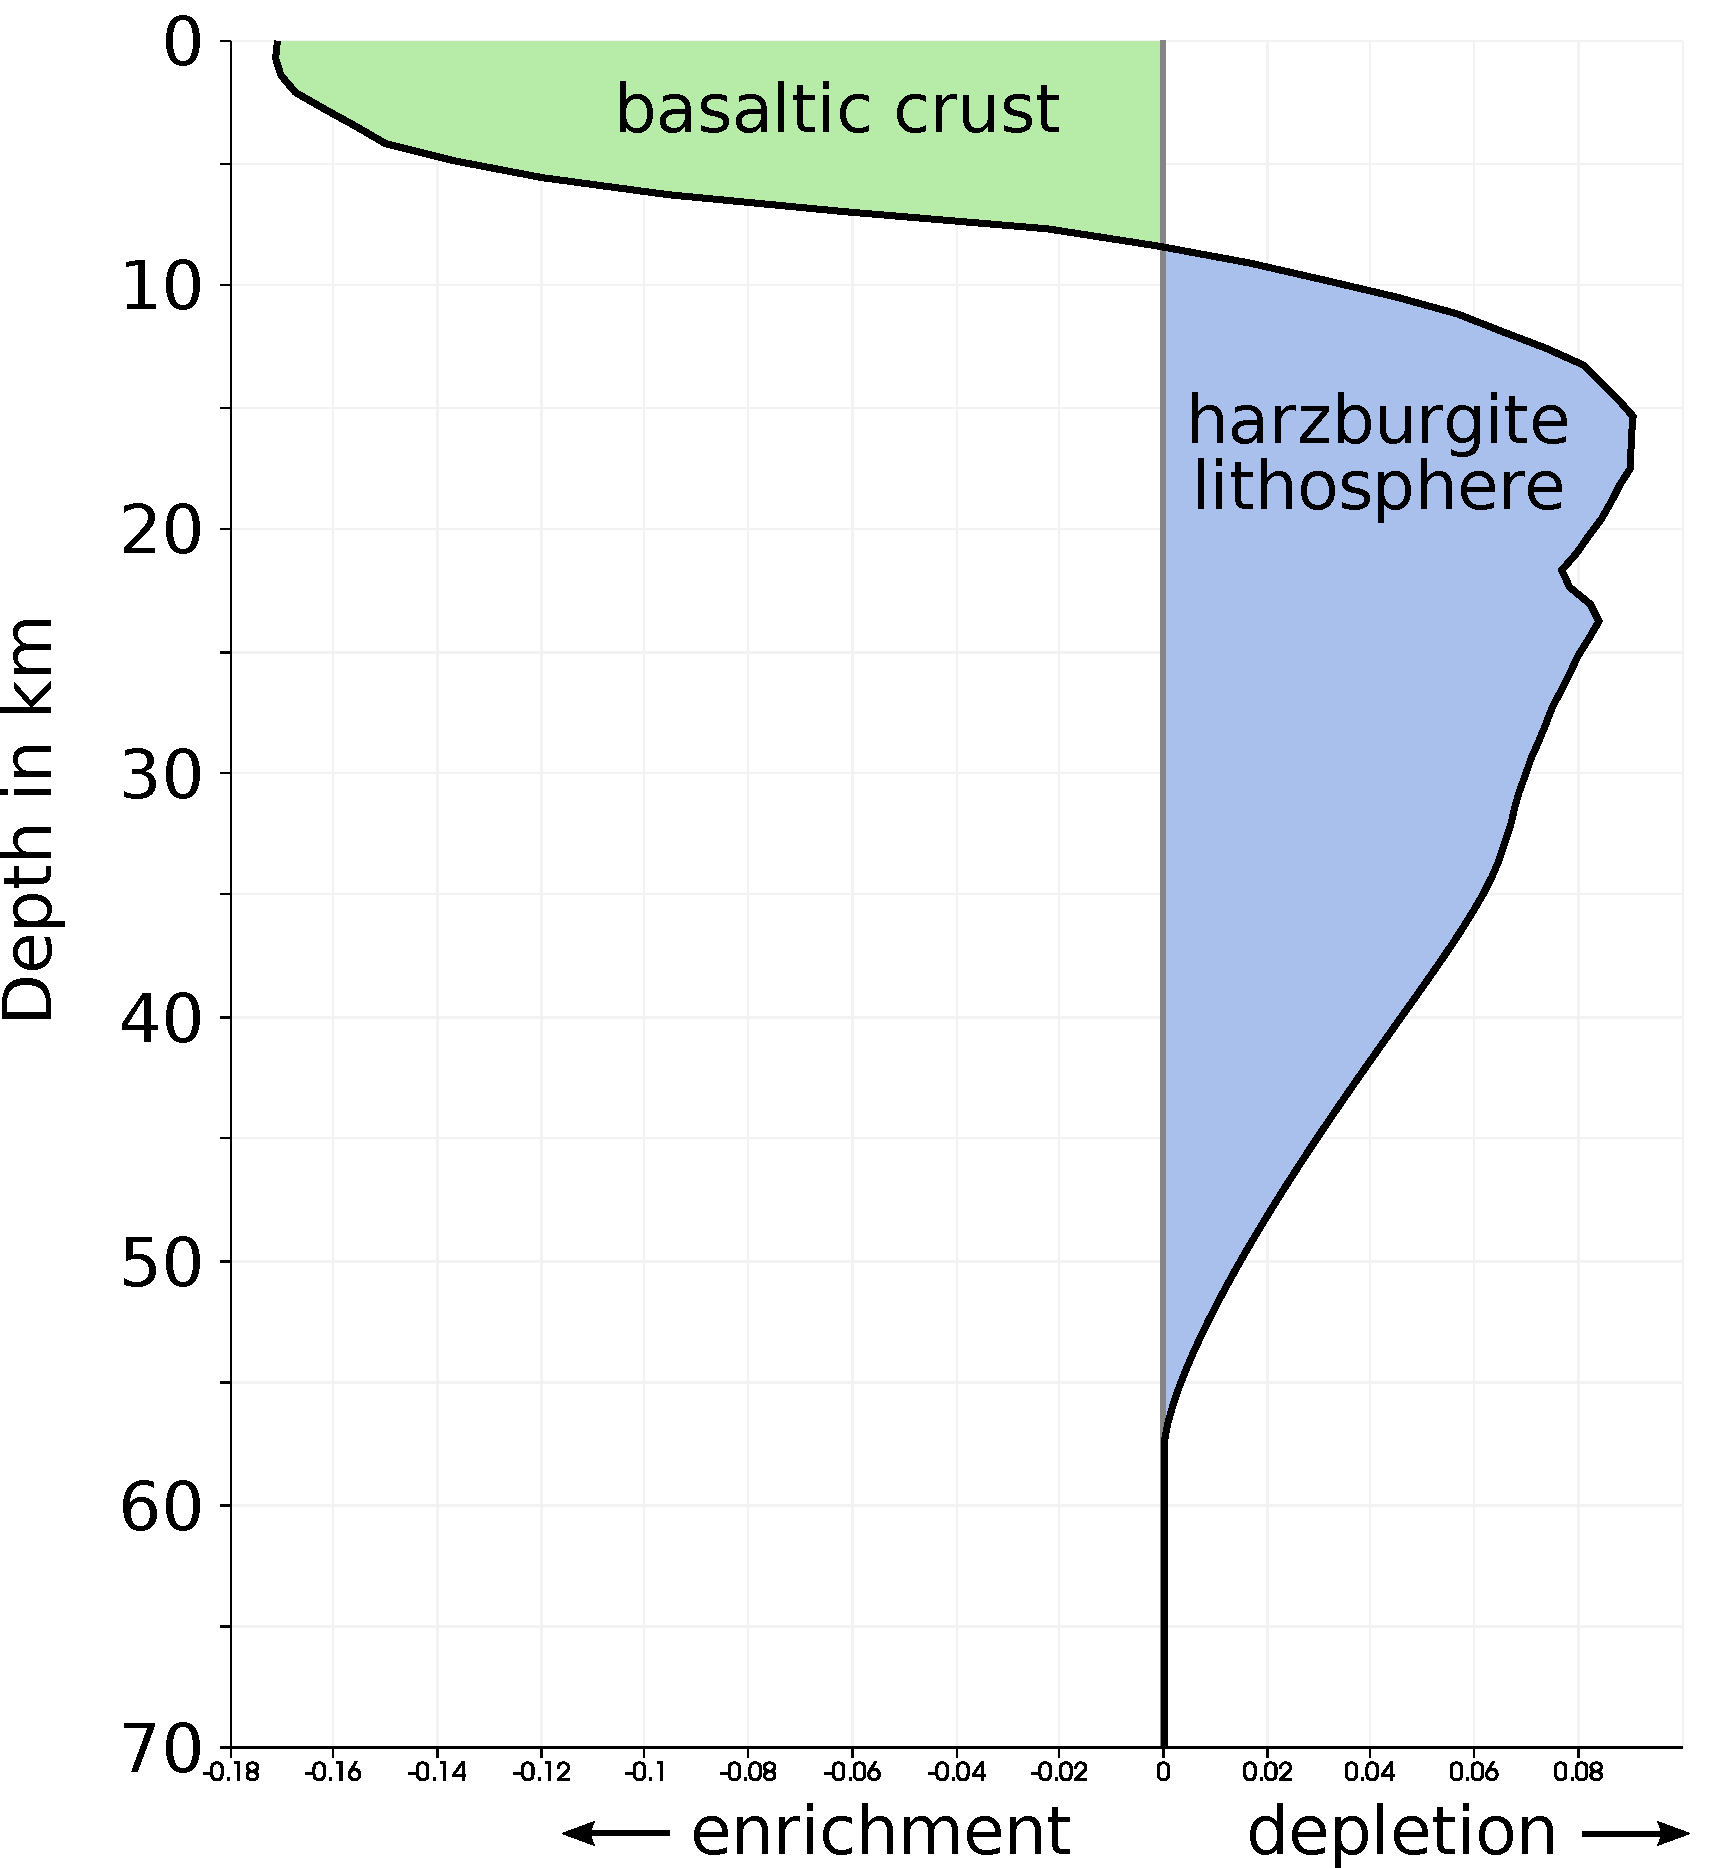
\includegraphics[width=0.35\textwidth]{cookbooks/mid_ocean_ridge/doc/depletion_profile.pdf}
    \caption{\it Vertical profile through the model domain at a distance of 80 km from the ridge axis
             at the end of the model run, showing the distribution of depletion and enrichment as
             indicated by the peridotite field.}
    \label{fig:mid-ocean-ridge-profile}
\end{figure}

\paragraph{Mesh refinement.}
Another option for making sure that melt migration is resolved properly in the model is using a
refinement criterion that directly relates to the compaction length. This can be done in the mesh
refinement section of the input file:

\lstinputlisting[language=prmfile]{cookbooks/mid_ocean_ridge/doc/compaction_length.part.prm.out}

This will lead to a higher resolution particularly in regions with low (but not zero) porosity,
and can be useful to resolve the strong gradients in the melt velocity and compaction pressure that
are to be expected in these places (see Figure~\ref{fig:mid-ocean-ridge-mesh}).
Of course it is also possible to combine both methods for refining the mesh.

\begin{figure}
    \centering
    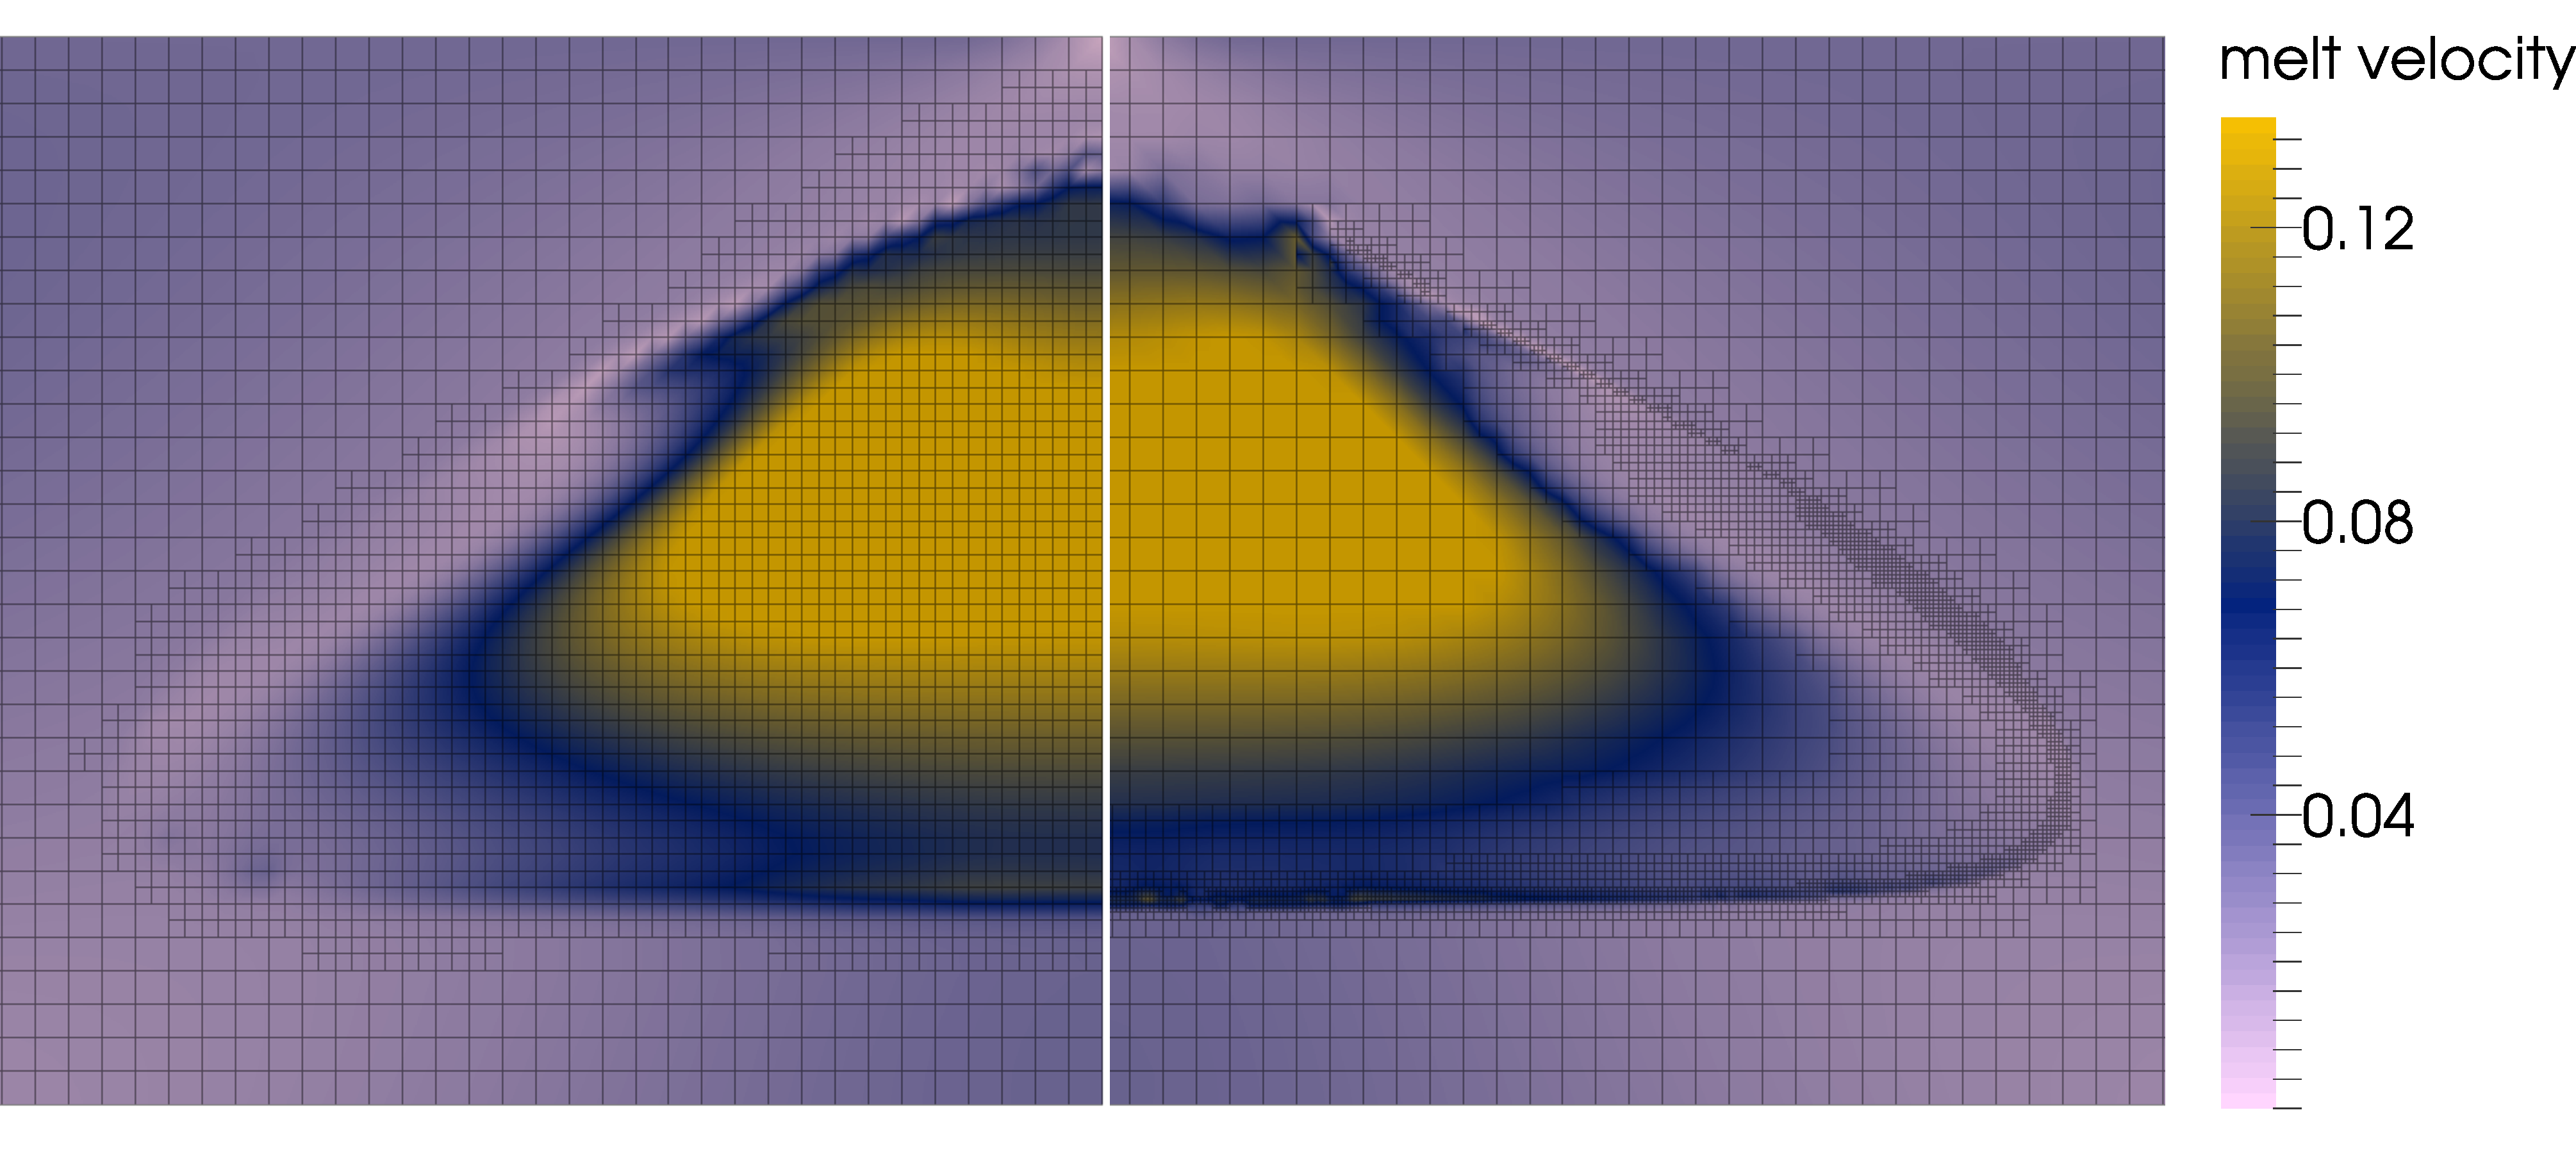
\includegraphics[width=0.6\textwidth]{cookbooks/mid_ocean_ridge/doc/refinement.pdf}
    \caption{\it Mesh after a time of 3.6 million years for a model using the composition threshold
             refinement strategy (left) and the compaction length refinement strategy (right)
             Background colors indicate the melt velocity. Its sharp gradients at the interface
             between regions with and without melt can only be resolved using the compaction
             length refinement strategy.}
    \label{fig:mid-ocean-ridge-mesh}
\end{figure}

\paragraph{Extending the model.}
There are a number of parameters that influence the amount of melting, how fast the melt moves, and ultimately the distribution of crustal and lithospheric material.
Some ideas for adapting the model setup:
\begin{itemize}
  \item Changing the spreading rate: This can be done by choosing a different magnitude of the
        prescribed velocity at the top boundary, and influences the size and shape of the triangular
        melting region. Faster spreading allows hot material to move further away from the ridge axis,
        and hence facilitates a melting region that extends further in horizontal direction.
  \item Changing the temperature profile: This can be done by choosing a different bottom boundary
        temperature and influences the amount of melting, and hence the thickness of the crust.
        Higher temperatures lead to more melt being generated.
  \item Changing the speed of melt migration: The velocity of the melt with respect to the solid velocity
        is determined by the permeability and the melt viscosity (and the pressure gradients in the melt).
        Increasing the permeability (by setting a different ``Reference permeability'' in the melt simple
        model) can lead to higher melt velocities, melt reaching the depth of freezing faster, and hence
        lower overall porosity values at steady state.
  \item Making the viscosity law more realistic: In this simple model, the viscosity only depends on the
        amount of melt that is present and is otherwise constant. This could be the reason why melt can
        not flow up all the way up at the ridge axis, but freezes before it reaches the surface.
        Introducing a temperature-dependent rheology could improve this behavior (and in reality, plastic
        effects might also play a role).
\end{itemize}
